%
% The first command in your LaTeX source must be the \documentclass command.
\documentclass[sigchi]{acmart}

%
% defining the \BibTeX command - from Oren Patashnik's original BibTeX documentation.
\def\BibTeX{{\rm B\kern-.05em{\sc i\kern-.025em b}\kern-.08emT\kern-.1667em\lower.7ex\hbox{E}\kern-.125emX}}
    
% Rights management information. 
% This information is sent to you when you complete the rights form.
% These commands have SAMPLE values in them; it is your responsibility as an author to replace
% the commands and values with those provided to you when you complete the rights form.
%
% These commands are for a PROCEEDINGS abstract or paper.
\copyrightyear{2026}
\acmYear{2026}
\setcopyright{acmlicensed}
\acmConference[SNA '26]{Social Network Analysis '26}{2025/26}{University of Pisa, Italy}
\acmBooktitle{Social Network Analysis '26}
\acmPrice{0.00}
%\acmDOI{10.1145/1122445.1122456}
%\acmISBN{978-1-4503-9999-9/18/06}


% end of the preamble, start of the body of the document source.
\begin{document}

%
% The "title" command has an optional parameter, allowing the author to define a "short title" to be used in page headers.
\title{Beyond Topics: Subcommunities in Substack's Recommendation Network}

%
% The "author" command and its associated commands are used to define the authors and their affiliations.
% Of note is the shared affiliation of the first two authors, and the "authornote" and "authornotemark" commands
% used to denote shared contribution to the research.
\author{Sara Rossi}
\email{s.rossi104@studenti.unipi.it}
\affiliation{%
  \institution{Student ID: 637107}
 }

\renewcommand{\shortauthors}{Rossi}


% The abstract is a short summary of the work to be presented in the article.
\begin{abstract}
Substack is a leading platform for independent publishing, where authors actively recommend other newsletters to their readership. Unlike algorithmic suggestions, these links represent deliberate editorial endorsements. While one might expect these endorsements to reflect shared subject matter, they may also signal shared views. This study investigates whether recommendation communities merely mirror newsletter topics or also capture affinities that topic labels miss. To address this, the recommendations were modeled as a network constructed via a breadth-first snowball crawl from 15 seed newsletters across five domains, yielding 15{,}186 nodes and 103{,}425 edges. Newsletter topics were inferred from post texts using TF--IDF and $k$-means clustering, while network communities were detected using the Louvain algorithm and validated for stability with Leiden. The analysis reveals a small-world, heavy-tailed network topology. Overall, recommendations strongly align with their topics: in domains like finance and food, a single community encompasses approximately 90\% of newsletters on that subject. However, where positions conflict, the topic alone is insufficient to explain network structure. Political newsletters fracture into three distinct communities (liberal mainstream, heterodox-centrist, and anti-establishment) that cut across finer sub-topics, and health newsletters critical of COVID-19 vaccines cluster with anti-establishment political commentary rather than with public-health publications.

\footnote{
\raggedright
{\bf Project Repositories}\\
\noindent Data Collection: \url{https://github.com/sara-rss/substack-recommendation-network/tree/main/data_collection}\\
\noindent Network Analysis: \url{https://github.com/sara-rss/substack-recommendation-network/tree/main/network_analysis}\\
\noindent Open Problem: \url{https://github.com/sara-rss/substack-recommendation-network/tree/main/open_problem}\\
}
\end{abstract}


%
% Keywords. The author(s) should pick words that accurately describe the work being
% presented. Separate the keywords with commas.
\keywords{Social Network Analysis, Substack, recommendation networks, community detection, homophily}


%
% This command processes the author and affiliation and title information and builds
% the first part of the formatted document.
\maketitle

\section{Introduction}
% ===================================================================
In recent years, many journalists, writers and experts have supplemented their work at traditional outlets with independent
publishing, often through newsletters delivered directly to subscribers' inboxes and supported by paid subscriptions. This shift means that part of public debate now takes place not in newspapers, which bring together many voices under one editorial line,
but in a fragmented landscape of individual authors, each addressing
their own audience. How these authors relate to one another is therefore an open question: whether they form communities of shared interests, or clusters of like-minded voices that rarely cross. On Substack, this
question can be observed directly, because authors publicly point their readers to other publications they value.

These recommendations are expected to follow subject matter, in the classic pattern of homophily~\cite{mcpherson2001birds}. Subject,
however, may not be the whole story: Adamic and Glance found that political blogs linked mostly to blogs with a similar orientation~\cite{adamic2005political}. This study asks \emph{whether the communities formed by recommendations simply mirror topics, or
whether in some domains they separate newsletters that write about the same subject}.


\section{Data Collection}
\label{sec:datacollection}
To study whether recommendations follow topics or positions, it was necessary to build a dataset that reflects both the recommendation choices of authors and the content of their newsletters.

\subsection{Selected Data Sources}

The data were collected from Substack, which makes publicly accessible
both the recommendations of each newsletter and its recent posts.
Recommendation lists were retrieved with the unofficial Python library
\texttt{substack-api}~\cite{substackapi}, and the most recent posts of each newsletter through the public \texttt{/api/v1/archive} endpoint. Substack does not, however, expose the category of newsletters run by other authors, so the topic of each newsletter had to be inferred from
its posts (see Node Attributes below). From these data, a network was built in which nodes are newsletters and a directed edge $A \to B$ indicates that $A$ recommends $B$.

The crawl began with 15 manually selected \emph{seed} newsletters, three
for each of five broad areas: literature, politics, technology, finance and health. Within each area, well-known and active newsletters were
chosen, so as to broaden thematic coverage and reduce the risk of
concentrating the crawl in a single niche. Each seed was checked for
active recommendations.

\subsubsection{Crawling Methodology and Assumptions}

The network was explored through snowball sampling, the only option in
the absence of a complete list of Substack publications. The crawl
proceeded breadth-first: for each newsletter it visited, the crawler
downloaded the full list of publications it recommends and added the
new ones to a queue, to be visited in turn.

The same newsletter may appear under slightly different URLs, for instance, with or without \texttt{www}, or with \texttt{http} rather than \texttt{https}. Each URL was therefore normalized before the network was constructed, ensuring that every newsletter corresponded to a single node.

To avoid overloading the platform, the crawler waited one second between
requests, and its progress was saved every 100 newsletters so that the
crawl could be resumed after any interruption. Despite these precautions,
the requests for 59 newsletters failed because of connection drops; they
were repeated in a second pass, and all of them were recovered. 

The network analyzed reflects three methodological choices:
\begin{itemize}
  \item \textbf{Induced subgraph.} Only expanded newsletters, whose recommendation lists were actually downloaded, are kept;
  recommendations pointing to the 38{,}525 newsletters discovered but
  never visited are discarded.
  \item \textbf{Static snapshot.} Recommendations were collected once,
  in August 2026, and the network describes the platform at that time.
  \item \textbf{Undirected graph.} The analyses use the undirected,
  unweighted version of the network. Since 41\% of recommendations are
  reciprocated, this discards the direction of the remaining 59\%.
\end{itemize}

\subsection{Node Attributes}
\label{sec:attributes}
The topic of each newsletter was inferred from the content of its posts. Titles and subtitles of the ten most recent posts were collected for every newsletter; 13{,}816 of the 15{,}186 newsletters (91\%) returned enough text to be analyzed. Topics were then identified in four steps:

\begin{enumerate}
\item \textbf{Language detection.} The language of each newsletter was detected with \texttt{langdetect}~\cite{langdetect,nakatani2010langdetect}. The 387 newsletters not in English (2.5\% of the network) were kept with language as a separate attribute, since a text model built for English would group them by language rather than by topic.
\item \textbf{Clustering.} After removing standard stopwords, numbers, dates, and generic newsletter terms, English texts were vectorized with TF--IDF~\cite{salton1988term} and clustered via $k$-means. Neither the elbow method nor the silhouette score points to an optimal number of clusters: across the values of $k$ tested between 5 and 30,
the inertia decreases steadily by only 1.5\%, without a clear elbow,
and the silhouette never exceeds 0.004, as is typical of sparse,
high-dimensional text vectors. The number of clusters was set to $k=16$, the smallest value where all five seed areas emerge as distinct clusters and health separates into its own topic.
\item \textbf{Recovery from post bodies.} Three clusters are weakly informative: generic titles, video and podcast episodes, and personal
  diaries. For their 5{,}097 members, the beginning of the post bodies was also downloaded; the 5{,}082 with enough body text were reassigned to the nearest existing centroid, without re-running $k$-means. This moved 1{,}246 newsletters to a more specific topic.
  \item \textbf{Keyword dictionary.} A dictionary of unambiguous keywords was applied to the newsletters remaining in these three clusters, only when at least 1\% of the words were topical and the first topic outweighed the second by a factor of 1.5. This moved 445 more.
\end{enumerate}

The resulting clusters were named by inspecting their most
characteristic terms and grouped into eight macro-topics
(Table~\ref{tab:topics}). Overall, 11{,}886 newsletters (78.3\%) have a
topic label. This figure includes the 1{,}863 newsletters left in the
\emph{personal} cluster, which is kept as a topic within lifestyle and
culture although it is only weakly informative; generic and video-only
newsletters are instead treated as having no topic. Since the area of
each seed was chosen in advance, the 15 seeds offer a small consistency
check: the classification, which ignores this information, assigns 12
of them to their area. Among the errors, Glenn Greenwald's newsletter publishes mostly video
episodes whose titles do not reveal their subject, a limit of
title-based topics discussed in Section~\ref{sec:discussion}.

\begin{table}[h]
  \centering
  \small
  \caption{Macro-topics inferred from post texts}
  \label{tab:topics}
    \begin{tabular}{@{}llr@{}}
    \toprule
    \textbf{Macro-topic} & \textbf{Topics} & \textbf{\%} \\
    \midrule
    Lifestyle \& culture & style and home, personal & 19.4 \\
    Arts \& letters      & writing, music           & 11.5 \\
    Technology           & AI, AI and coding        & 11.4 \\
    Politics             & US, UK, geopolitics      & 10.9 \\
    Finance              & equity, macro            & 10.2 \\
    Business             & business                 & 7.4 \\
    Science \& health    & health                   & 4.7 \\
    Food                 & food                     & 2.8 \\
    \midrule
    No topic             & generic, non-English, video & 12.7 \\
    No text              &                          & 9.0 \\
    \bottomrule
  \end{tabular}
\end{table}

\section{Network Characterization}
\label{sec:network}

The final network comprises 15{,}186 newsletters and 103{,}425
recommendations. As explained in Section~\ref{sec:datacollection}, all
measures are computed on the undirected version of the graph, which
contains 82{,}062 edges.


\subsection{Degree Distribution}
\label{sec:degree}

Connectivity is highly unequal. The degree ranges from 1 to 380, with a mean of 10.81 but a median of only 6: 15\%
of newsletters have a single connection, while a few hubs reach several
hundred. At most 50 outgoing recommendations per newsletter are available, so
high degrees are driven by recommendations received: for the three largest hubs, over 90\% of connections are incoming. Heather Cox Richardson's \emph{Letters from an American}, a political newsletter, has the highest degree and is recommended by 377 other newsletters. Other prominent hubs focus on venture capital, start-ups, artificial intelligence, and finance.


\begin{figure*}[t]
  \centering
  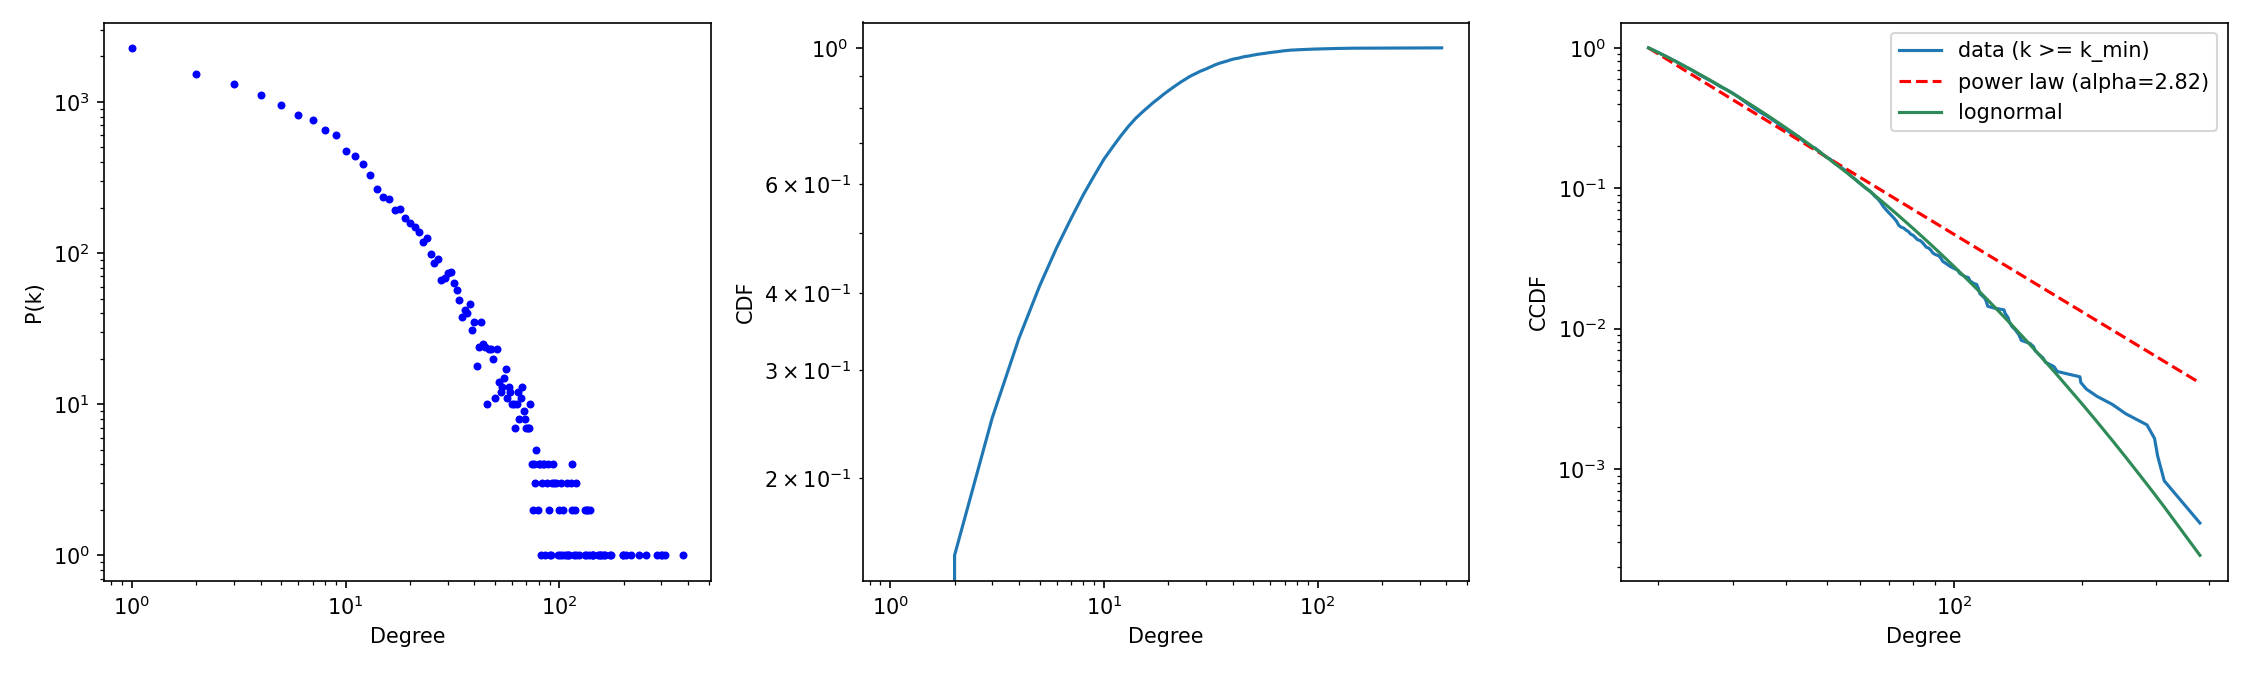
\includegraphics[width=\textwidth]{img/grado_distribuzione.png}
  \caption{Degree distribution: $P(k)$ on a log-log scale (left),
  cumulative distribution (center), and complementary cumulative
  distribution of the tail ($k \geq 19$) with the fitted power law and
  lognormal (right).}
  \label{fig:degree}
\end{figure*}

The degree distribution was examined through the three panels of Figure \ref{fig:degree}:

\begin{itemize}
  \item in the log-log plot (left), $P(k)$ bends downwards as the degree
  increases;
  \item the cumulative distribution (center) shows that about two thirds
  of newsletters have fewer than ten connections;
  \item the tail was fitted with the \texttt{powerlaw} package. The best
power law ($k_{\min}=19$, $\alpha=2.82$, with $P(k) \propto k^{-\alpha}$)
is outperformed by both a lognormal and a truncated power law
($p<10^{-6}$), but outperforms an exponential ($p=0.036$). In the
complementary cumulative distribution (right), the power law departs from
the data around $k=40$, while the lognormal follows them up to the
largest hubs.
\end{itemize}
The distribution is therefore heavy-tailed but not scale-free in the
strict sense. The network is also mildly disassortative ($r=-0.081$),
a pattern common in information networks~\cite{newman2002assortative}
that may partly reflect the asymmetry of recommendations.


\subsection{Components and Paths}
\label{sec:paths}

The network forms a single connected component, a result that reflects the snowball sampling, which only reaches newsletters linked to
the seeds. Shortest paths were computed between all pairs of nodes. The average shortest path is 4.34 and the diameter of the network is 9, but long
paths are rare: 41\% of pairs are at distance 4, and 91\% are at most five steps apart. Thus most newsletters can be connected through a short chain of recommendations.

\subsection{Density and Clustering}
\label{sec:clustering}

The network density is 0.00071, making the network very sparse: on
average, each newsletter is connected to fewer than 0.1\% of the others.
The average clustering coefficient is 0.151, modest in absolute terms,
and it declines steadily with degree, from 0.25 among newsletters with
two to five connections to 0.03 among those with more than one hundred.
Thus, lower-degree newsletters tend to have more tightly knit
neighborhoods, whereas the neighbors of hubs are rarely connected to
one another.

The network contains 57{,}649 triangles. Its global transitivity (0.064) is lower than the average clustering, a difference that may reflect open triads around hubs: several newsletters are connected to the same hub without being connected to one another, so hubs contribute many connected triples, most of which remain open. 

\subsection{Centrality Analysis}
\label{sec:centrality}

Three centrality measures were computed: \emph{degree},
\emph{betweenness} and \emph{closeness} (Table~\ref{tab:centrality}). To compare them, Spearman's rank correlation $\rho$
was used, which measures how similar the rankings produced by two
measures are. 

Betweenness is strongly correlated with degree ($\rho=0.913$), while closeness departs more from it ($\rho=0.827$): next
to the largest hubs, it brings out four newsletters that are not among the most connected: Paul Krugman's newsletter,
\emph{The Free Press}, \emph{Noahpinion} and \emph{The Honest Broker}, all offering commentary on politics, economics or culture rather than on a single niche.

A central position, however, can have two different meanings. A
newsletter may be central because it links different parts of the
network, or simply because it sits in the middle of one large
community. To tell the two cases apart, the participation coefficient
$P = 1 - \sum_c (k_c/k)^2$ was computed, where $k_c$ is the number of
neighbors in community $c$: $P$ is 0
when all the neighbors of a newsletter belong to one community, and
approaches 1 when they are spread across many. Its median is 0.30 for
newsletters with 30 to 120 connections and 0.40 for the ten largest
hubs. The four high-closeness newsletters above range from 0.69 to
0.76, with neighbors in eight or nine of the ten main communities: they
are close to the rest of the network because they are connected to all
of its parts.

The same measure separates two kinds of newsletters with high
betweenness:
\begin{itemize}
  \item \textbf{Bridges between communities.} The newsletters of Junot
  D\'iaz, Seymour Hersh and Adam Grant have a moderate degree but a high
  participation (0.57 to 0.77): their neighbors are spread across
  communities, so the shortest paths that cross them connect different
  parts of the network.
  \item \textbf{Brokers within a community.} \emph{Why Is This
  Interesting?} also ranks high by betweenness (50th), but 81\% of its
  neighbors belong to its own community ($P=0.34$): it lies on many
  shortest paths, but mostly within that community.
\end{itemize}
High betweenness therefore marks a bridge between communities only
when it comes with high participation.

\begin{table*}[t]
  \centering
  \caption{Top 10 newsletters by degree, betweenness and closeness.}
  \label{tab:centrality}
  \begin{tabular}{lrlrlr}
    \toprule
    \multicolumn{2}{c}{\textbf{Degree}} & \multicolumn{2}{c}{\textbf{Betweenness}} & \multicolumn{2}{c}{\textbf{Closeness}} \\
    \midrule
    heathercoxrichardson & 380 & heathercoxrichardson & 0.044 & heathercoxrichardson & 0.333 \\
    thevccorner & 313 & vitaliy & 0.030 & auraist & 0.325 \\
    22ndcenturyfrontier & 302 & thevccorner & 0.029 & paulkrugman & 0.316 \\
    the-founders-corner & 297 & auraist & 0.027 & vitaliy & 0.315 \\
    themarketdispatch & 285 & ai-supremacy & 0.027 & thevccorner & 0.314 \\
    ai-supremacy & 254 & 22ndcenturyfrontier & 0.023 & ai-supremacy & 0.314 \\
    vitaliy & 236 & the-founders-corner & 0.021 & thefp & 0.311 \\
    oldster & 217 & neweconomies & 0.016 & honest-broker & 0.310 \\
    neweconomies & 205 & doomberg & 0.015 & the-founders-corner & 0.309 \\
    macromornings & 199 & thefp & 0.015 & noahpinion & 0.308 \\
    \bottomrule
  \end{tabular}
\end{table*}



\subsection{Comparison with ER}
\label{sec:er}
The properties described above were compared with those of two
reference models with the same number of nodes, each generated ten
times, in order to identify which of them go beyond chance
(Table~\ref{tab:models}).

The first model is an Erd\H{o}s--R\'enyi (ER) random graph, generated with a
fixed number of edges so that it matches the real network. In this model
every pair of nodes is equally likely to be connected, with a
corresponding probability $p = 2L/n(n-1) = 7.1 \times 10^{-4}$, where
$L$ is the number of edges, which lies above both the threshold for the emergence of a giant component, $p_c = 1/n = 6.6 \times 10^{-5}$, and the connectivity threshold, $\ln n / n = 6.3 \times 10^{-4}$. The ER graph is therefore in the \emph{connected regime}, although close to its boundary, with 1.6 components on average. At this density an almost connected graph is thus expected by chance: the connectedness of the real network is not a distinctive feature, and is in any case favored by the sampling.

The same holds for distances: the average shortest path of the ER graph
(4.32) is almost identical to the real one (4.34), although the real
network has a larger diameter (9 against 7). The two differ, instead, in how
connections are distributed. In the ER graph degrees follow a Poisson
distribution concentrated around the mean, with a maximum of 27 against
380 in the real network, so there are no hubs (Figure~\ref{fig:models})
and no correlation between the degrees of connected nodes
(assortativity 0.00 against $-0.08$). Its clustering is also about 200
times lower, since two neighbors of a node are no more likely to be
connected than any other pair. Randomness alone therefore accounts for
the connectivity and the short paths of the real network, but neither
for its hubs nor for its clustering.


\begin{table}[h]
  \centering
  \caption{Comparison between the real network and the theoretical
  models (ER, BA). Model values are averages over 10 realizations.}
  \label{tab:models}
  \begin{tabular}{lccc}
    \toprule
    \textbf{Metric} & \textbf{Real network} & \textbf{ER} & \textbf{BA} \\
    \midrule
    Nodes                  & 15{,}186 & 15{,}186 & 15{,}186 \\
    Edges                  & 82{,}062 & 82{,}062 & 75{,}905 \\
    Average degree         & 10.8     & 10.8     & 10.0 \\
    Maximum degree         & 380      & 27       & 470 \\
    Connected components   & 1        & 1.6      & 1 \\
    Average clustering     & 0.1509   & 0.0007   & 0.0051 \\
    Avg.\ shortest path    & 4.34     & 4.32     & 3.78 \\
    Diameter               & 9        & 7        & 6 \\
    Degree assortativity   & $-0.08$  & 0.00     & $-0.02$ \\
    \bottomrule
  \end{tabular}
\end{table}

\subsection{Comparison with BA}
\label{sec:ba}

The second model is a Barab\'asi--Albert (BA) graph, in which new nodes
attach preferentially to well-connected ones. Since its parameter $m$
must be an integer, $m=5$ was used, as it gives the number of edges
closest to the real network; $m=6$ leads to the same conclusions
(clustering 0.0057, average shortest path 3.60).

Preferential attachment reproduces the heavy tail that the ER model
lacks, but not its shape. It overestimates the hubs (maximum degree 470
against 380), consistent with a real tail that bends below a pure power
law, and it has no periphery: every node
enters with $m$ links, so the minimum degree is 5, whereas 15\% of the
newsletters have a single connection (Figure~\ref{fig:models}). The BA
graph is also more compact than the real network, with shorter paths
(3.78 against 4.34) and a smaller diameter (6 against 9), and it is
less disassortative ($-0.02$ against $-0.08$). The main difference,
however, concerns clustering, which is still about thirty times lower
than in the real network.

Taken together, the two comparisons show that the network is a
small-world network: it combines the short paths of a random graph with
a clustering about two hundred times higher than in the random graph.
A preferential-attachment model reproduces the hubs, but not this local
structure. Recommendations do not merely target popular newsletters: while major
hubs rarely reciprocate, 41\% of all recommendations are mutual,
suggesting frequent exchange between peers.
Section~\ref{sec:openquestion} examines whether the local structure of
the network reflects topics.


\begin{figure}[h]
  \centering
  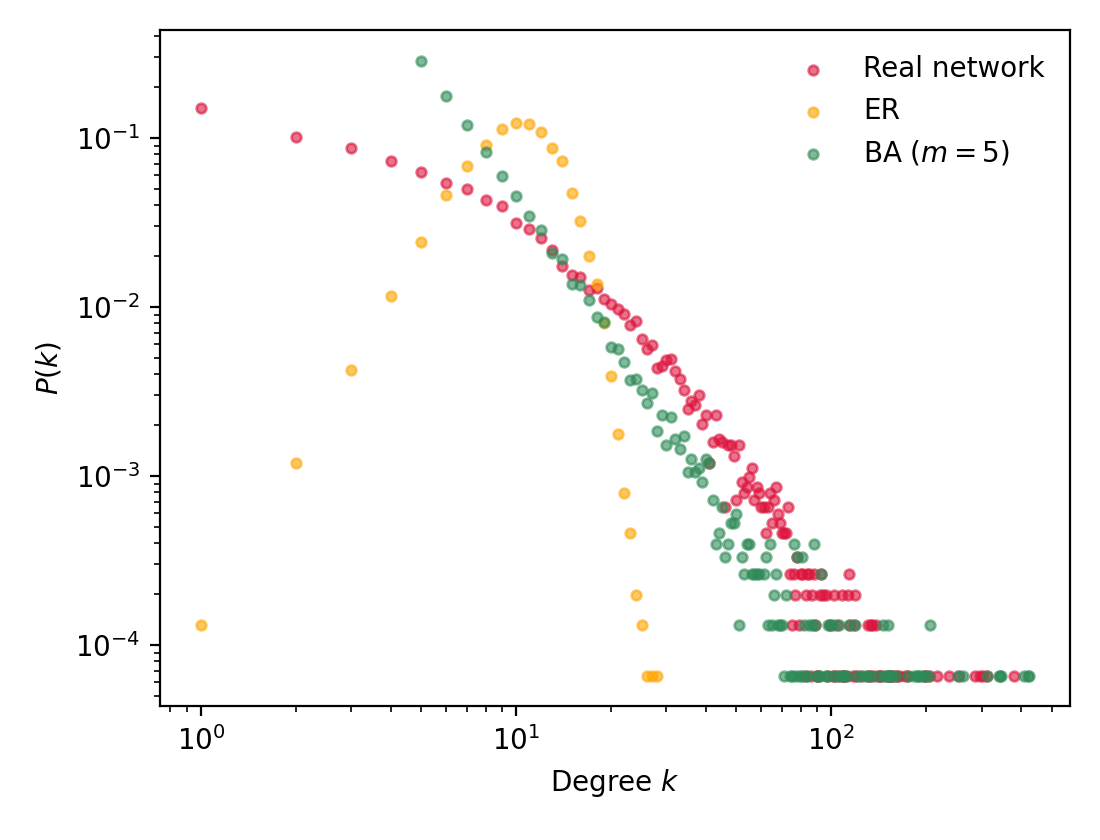
\includegraphics[width=0.75\linewidth]{img/confronto_gradi.png}
  \caption{Degree distribution $P(k)$ of the real network compared to the Erd\H{o}s--R\'enyi (ER) and Barab\'asi--Albert (BA, $m=5$) theoretical models on logarithmic scales.}
  \label{fig:models}
\end{figure}


\section{Open Question}
\label{sec:openquestion}

\subsection{Approach}
Having characterized the structure of the network, the analysis turns
to its central question: \emph{do newsletters recommend what they write
about, or also whom they agree with?} The clustering observed in
Section~\ref{sec:network} suggests that the network is organized in
dense groups. The question is whether these groups simply correspond to
topics, or whether recommendations also reflect affinities that topic
labels miss, such as a shared political stance.

The same newsletters are grouped twice, in two independent ways:
\begin{itemize}
  \item \textbf{by recommendations}: communities detected from the
  network alone, ignoring content;
  \item \textbf{by content}: topics inferred from texts alone, ignoring
  recommendations.
\end{itemize}
If newsletters recommended only what they write about, the two
groupings would largely coincide; where they diverge, the network
reveals something that texts alone do not. The comparison is carried
out both against a null model that randomly permutes topic labels among
nodes and through the inspection of individual communities. Newsletters
without a topic label are excluded from the comparison, and their
distribution is analyzed separately.

\subsection{Communities and Their Stability}
Communities were detected with the Louvain algorithm, which maximizes
modularity. Since Louvain is stochastic, it was run 30 times with
different seeds, and the partition most similar on average to the
others, measured by normalized mutual information (NMI), was kept as
reference. It contains 21 communities, with a modularity of 0.641. The
ten largest cover 97.5\% of the newsletters (Figure~\ref{fig:network});
the other eleven are marginal, with 384 newsletters in total.

To assess how much the result depends on the algorithm, the reference
partition was compared with 30 further runs of Louvain and 30 runs of
Leiden, which guarantees well-connected communities. Agreement is
substantial but not complete (NMI 0.73 with Louvain and 0.70 with
Leiden): the overall structure is robust, while the boundaries between
some communities vary. Table~\ref{tab:communities} reports, for each
community, its \emph{cohesion}, that is, the probability that two of its members end up in the same community in another run. 

The most stable communities highlight the network's sharp boundaries. While finance and entrepreneurship might intuitively overlap, they form distinct, highly reproducible groups: \emph{investing} (cohesion 0.90) contains 90\% of finance newsletters, whereas \emph{start-ups and
technology} (0.83) gathers over 60\% of business and technology ones. Both keep roughly three quarters of their edges internal (79\% and
75\%). Conversely, the \emph{health and science} (0.53), \emph{heterodox-centrist } (0.55) and \emph{literary} (0.56) communities are the least stable among the larger ones, with members frequently split across different communities
between runs.

\subsection{Communities and Topics}
\label{sec:commtopics}

The overlap between communities and topics was measured on the
11{,}886 newsletters with a topic label, using three measures:
\begin{itemize}
  \item \emph{topical assortativity}, on the macro-topics: whether
  recommendations connect newsletters on the same topic more often than
  random links would;
  \item \emph{normalized mutual information} (NMI): how much the
  community of a newsletter reveals about its topic;
  \item \emph{homogeneity} and \emph{completeness}: whether each
  community contains a single topic, and whether each topic falls within
  a single community.
\end{itemize}

To check that this overlap is not a matter of chance, topic labels were
shuffled at random among the newsletters, leaving the network and the
communities unchanged, 500 times for NMI and 50 for assortativity.

Communities and topics match far more closely than chance would allow.
Assortativity is 0.49 and NMI 0.36, whereas the shuffled labels give
values close to zero ($-0.001 \pm 0.002$ and $0.003 \pm 0.0003$).
Communities found from the links alone therefore reveal a great deal
about what newsletters write about.

Yet topic does not explain everything. Homogeneity (0.38) and
completeness (0.35) are both far from 1, which means that the match
fails in two ways:
\begin{itemize}
    \item \textbf{Communities mix topics} (low homogeneity). Even in the purest community, music, film and pop culture, the dominant topic
  covers only 72\% of the labeled members; in the heterodox-centrist
  community it covers 41\% (purity in Table~\ref{tab:communities}).
  \item \textbf{Topics are spread over several communities} (low
  completeness). Finance and food newsletters each fall almost entirely
  within a single community (90\% and 91\%), whereas politics is split
  across three (45\%, 24\% and 18\%), and science and health is the most
  scattered, with only 41\% in its main community.
\end{itemize}

\begin{table*}[t]
  \caption{The ten main communities by size, showing purity (share of the
  dominant macro-topic) and cohesion (pairwise co-assignment stability under
  Louvain and Leiden). Newsletters are identified by their URL.}
  \label{tab:communities}
  \small
  \setlength{\tabcolsep}{4pt}
  \begin{tabular*}{\textwidth}{@{\extracolsep{\fill}}lrlrrl@{}}
    \toprule
    Community & Nodes & Dominant macro-topic & Purity & Cohesion & Central newsletters \\
    \midrule
    Start-ups \& technology    & 2{,}701 & technology           & 49\% & 0.83 & the-founders-corner, thevccorner \\
    Literary \& personal essay & 2{,}667 & lifestyle \& culture & 50\% & 0.56 & oldster, georgesaunders \\
    Investing                  & 2{,}577 & finance              & 70\% & 0.90 & themarketdispatch, macromornings \\
    Food, fashion \& home      & 1{,}730 & lifestyle \& culture & 56\% & 0.64 & thesecretingredient, davidlebovitz \\
    Liberal mainstream         & 1{,}545 & politics             & 66\% & 0.69 & heathercoxrichardson, robertreich \\
    Heterodox-centrist         & 1{,}398 & politics             & 41\% & 0.55 & thefp, andrewsullivan \\
    Anti-establishment         &    738  & politics             & 56\% & 0.72 & merylnass, racket.news \\
    Health \& science          &    723  & science \& health    & 48\% & 0.53 & yourlocalepidemiologist, insidemedicine \\
    Music, film \& pop culture &    611  & arts \& letters      & 72\% & 0.66 & bradkyle, thekevinalexander \\
    Heterogeneous              &    112  & lifestyle \& culture & 52\% & 0.39 & coolstoriesabout.art, leaderunlock \\
    \bottomrule
  \end{tabular*}
\end{table*}

\begin{figure*}[t]
  \centering
  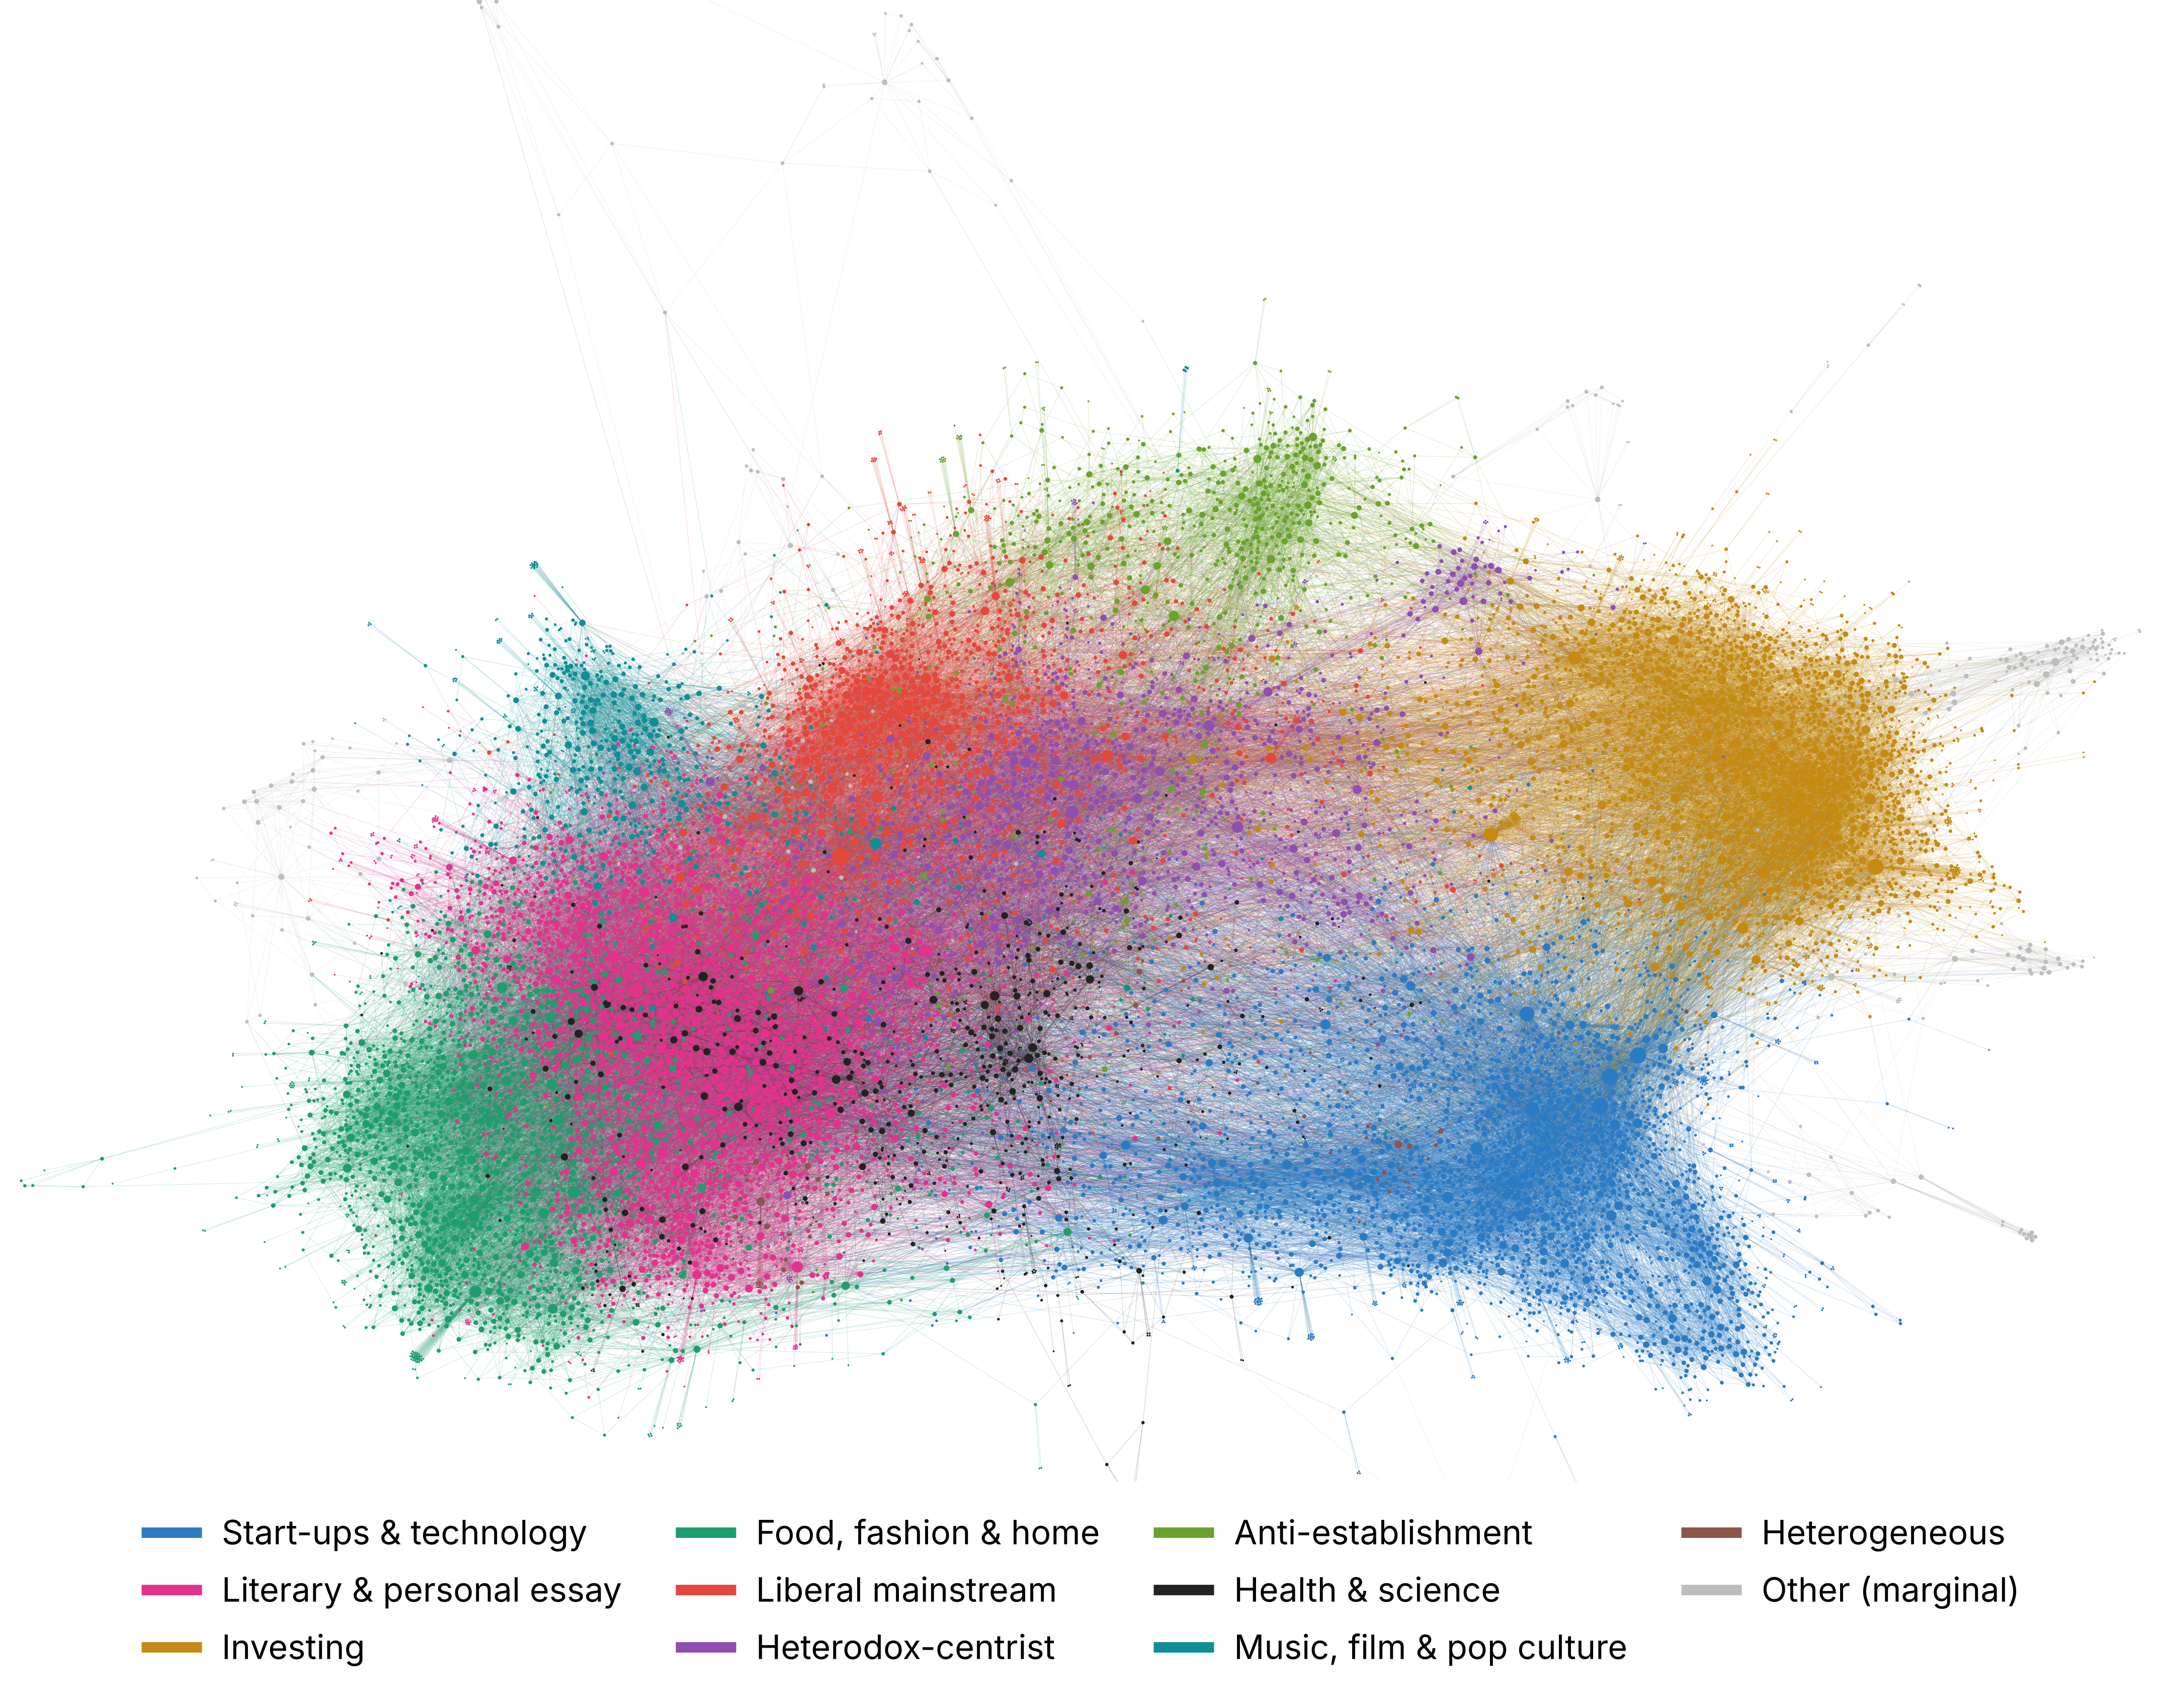
\includegraphics[width=\textwidth]{img/grafo_finale.png}
  \caption{The recommendation network, with newsletters colored by community.}
  \label{fig:network}
\end{figure*}

\subsection{Where Topic Is Not Enough}
\label{sec:stance}

Politics is the clearest case of a topic split across communities. Most
political newsletters fall into three communities:
\begin{itemize}
  \item \textbf{Liberal mainstream} (\emph{Letters from an American},
  Robert Reich, \emph{The Bulwark}): commentary critical of Donald
  Trump, mostly from the center-left but also from former Republicans.
  \item \textbf{Heterodox-centrist} (\emph{The Free Press}, Andrew
  Sullivan, \emph{Slow Boring}, \emph{Noahpinion}): writers who reject
  partisan orthodoxies on either side, especially progressive positions on cultural issues.
  \item \textbf{Anti-establishment} (Chris Hedges, \emph{Racket News}, Caitlin Johnstone): critics of mainstream institutions, media and US foreign policy, drawn from both the left and the right.
\end{itemize}
The liberal and anti-establishment blocks are among the more stable communities (cohesion 0.69 and 0.72), while the heterodox-centrist one is the least stable of the three political communities (0.55). The anti-establishment community, although the smallest, is also the
most inward-looking of the three, keeping 61\% of its edges internal.

The split cannot be explained by finer political topics, since the text-based political clusters cut across the three communities:
\begin{itemize}
  \item \textbf{US politics}: most newsletters fall in the liberal
  community (63\%), but 14\% belong to the anti-establishment one and
  13\% to the heterodox one.
  \item \textbf{Geopolitics}: newsletters are divided between the
  liberal (47\%) and the anti-establishment community (30\%).
  \item \textbf{UK politics}: the only partial alignment, with half of
  the cluster in the heterodox community. Its most connected members,
  however, mix British commentators with American policy writers,
  suggesting that the cluster captures a register of policy commentary
  as much as a country.
\end{itemize}


Health shows a similar pattern. \emph{Science and health} is the most
scattered macro-topic, and its two largest shares fall in two different communities:
\begin{itemize}
  \item \textbf{Health and science} (41\% of health newsletters): built
  around public-health and medical newsletters such as \emph{Your Local
  Epidemiologist} and \emph{Inside Medicine}.
  \item \textbf{Anti-establishment} (11\% of health newsletters): of the
  fifteen most connected among them, 13 publish content critical of
  COVID-19 vaccines, vaccine mandates or the public-health institutions
  that promoted them, such as Steve Kirsch's newsletter and
  \emph{Popular Rationalism}; the other two deal with nutrition and
  general wellness.
\end{itemize}
These vaccine-critical newsletters share a topic label with the
public-health newsletters, yet they are recommended alongside
anti-\hspace{0pt}establishment political commentary rather than
alongside other health newsletters. In
Figure~\ref{fig:network}, the two communities lie far apart: the
anti-establishment community on the upper edge of the network, the
health and science community near its center.
In both domains, then, the topic assigned from text is correct but
insufficient: the network separates newsletters that write about the
same subject from different positions.


\subsection{Missing Labels}
\label{sec:missing}

Of the 15{,}186 newsletters, 3{,}300 (21.7\%) have no topic label:
1{,}403 have only generic titles, 1{,}370 have no retrievable text, 387 are not in English and 140 publish mostly video. These newsletters are left without a topic in all the analyses above. The question is therefore: \emph{are newsletters without a topic scattered across the network, or concentrated in some parts of it?} If they are scattered, the results above hold for the whole network; if they are concentrated, the parts where they gather are described less reliably.

To answer this question, the distribution of missing labels was analyzed at two levels:
\begin{itemize}
  \item \textbf{Degree.} As shown in Figure~\ref{fig:missing}, missing
  labels are concentrated among weakly connected newsletters: the share without a label falls from 35.9\% among newsletters with a single connection to 13.0\% among those with more than 50. Results show that unlabeled newsletters have fewer connections than labeled ones (median degree 4 against 7), and a Mann--Whitney test confirms that this difference is not due to chance ($p < 10^{-88}$).
  
  Among newsletters with a single connection,
  more than half of the missing labels are due to the absence of text
  rather than to uninformative titles, which suggests inactive publications or failed downloads.
  \item \textbf{Communities.} The 384 newsletters outside the ten main
  communities lack a label in 68.5\% of cases. Within the main
  communities, the share of missing labels also varies: it ranges from
  12.4\% in the food, fashion and home community to 41.1\% in the
  heterogeneous one, and lies between 25.8\% and 29.3\% in the three
  political communities. A $\chi^2$ test confirms that these
  differences are not due to chance ($p < 10^{-50}$), although they
  are modest in size (Cramér's $V = 0.14$).
\end{itemize}
Missing labels therefore mainly affect the periphery of the network
and, to a lesser extent, some communities (e.g.\ the political ones).

\subsubsection{Side analysis: can communities suggest missing topics?}
It was checked whether community membership indicates the likely topic of an unlabeled newsletter. On the labeled newsletters of the ten main communities, hiding each label and comparing it with the dominant topic of its community gives 55.8\% agreement, against 15.4\% by chance and 24.8\% when always choosing the most frequent topic. Agreement rises to 68.8\% in the three purest communities (investing, liberal mainstream, music, film and pop culture), but remains weak in mixed ones such as the heterodox-centrist, anti-establishment and heterogeneous
communities.

\begin{figure}[h]
  \centering
  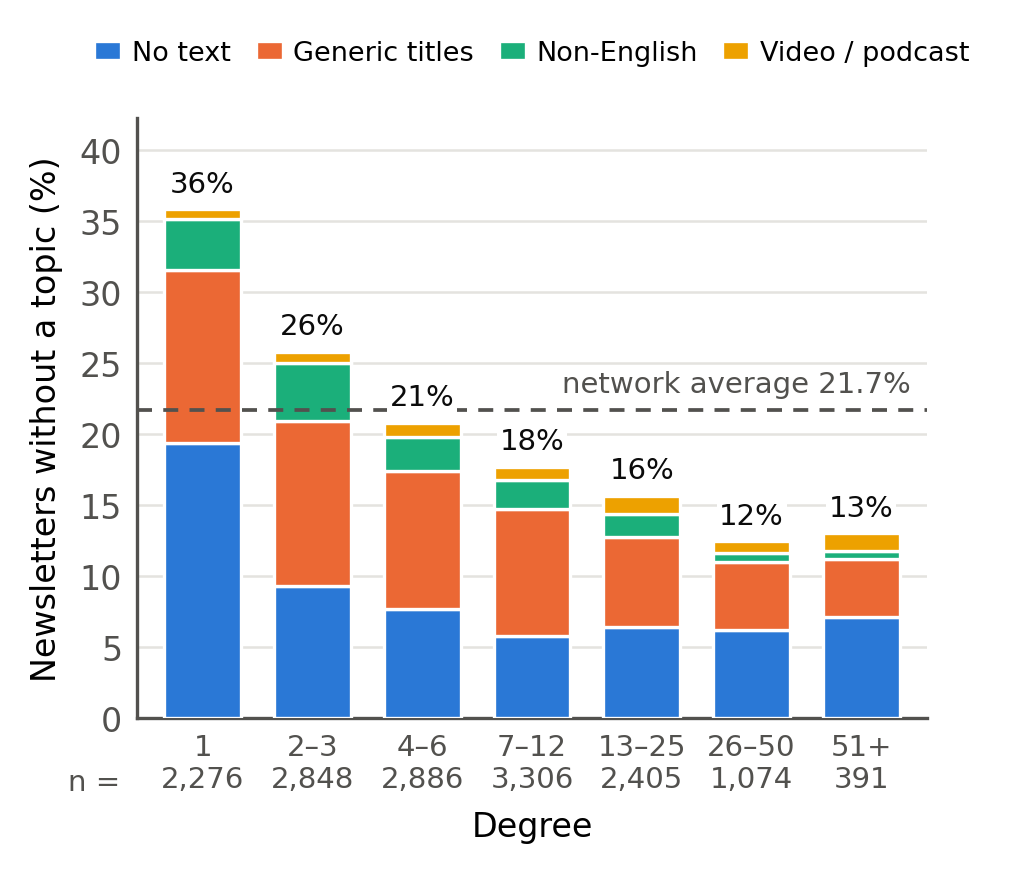
\includegraphics[width=\columnwidth]{img/label_mancanti_grado.png}
  \caption{Unlabeled newsletters by degree band and cause of missing label.}
  \label{fig:missing}
\end{figure}


\section{Discussion}
\label{sec:discussion}

This study asked whether Substack recommendations reflect shared
subject matter or also capture affinities that topic labels miss. The
answer is that they do both, depending on the domain. Topic is the
dominant organizing principle: recommendations stay within the same
topic far more often than chance would predict, and in domains such as
finance and food a single community gathers almost all the newsletters
on that subject. Where positions conflict, however, topic is no longer
enough. Political newsletters split into three communities that cut
across their finer topics, and health newsletters critical of COVID-19
vaccines are recommended alongside anti-establishment political
commentary rather than alongside public-health newsletters.

These results extend the observation of Adamic and
Glance~\cite{adamic2005political}, who found that political blogs link
mostly within their own orientation, in three directions. First, the
division emerges without any prior labelling: communities were detected
from recommendations alone, and stance appeared only on inspection.
Second, it is not limited to two opposing camps, since heterodox-centrist
newsletters form a community of their own. Third, it appears outside
politics: in health, the network separates newsletters on the same
subject according to their position.

In the terms of
McPherson et al.~\cite{mcpherson2001birds}, recommendations combine
homophily based on what newsletters write about with homophily based
on the values they express. The anti-establishment community is a clear example: its most central newsletters include left-wing critics of US foreign policy and media as well as vaccine-critical health newsletters, which suggests that what holds it together is a shared distrust of mainstream institutions rather than a
common subject or a position on the left--right axis.

The structural analysis is consistent with this interpretation. The network
is a small world whose hubs are built by recommendations received, and
its clustering is about 200 times higher than in a random graph and 30 times higher than under preferential attachment. Popularity alone, which preferential attachment captures, does not explain the local structure; the community analysis shows that this structure largely follows topic, and in contested domains follows stance.

\subsection{Limitations}
The study has several limitations.
\begin{itemize}
   \item \textbf{Sampling.} The snowball crawl reaches only newsletters connected to the seeds and favors well-recommended ones. Newsletters discovered late have fewer known connections, so centrality partly reflects the order of the crawl.
  \item \textbf{Snapshot and direction.} Since the network is a single snapshot analyzed as undirected, it cannot show how recommendations change over time, nor whether they flow mostly in one direction between communities.
  \item \textbf{Topics from titles.} Topics were inferred from titles, subtitles and the beginning of a few posts, with clusters that are
  only weakly separated. Some labels are vague (\emph{personal}) or imprecise (\emph{UK politics}), and newsletters that publish mostly video or have generic titles cannot be classified.
  \item \textbf{Missing labels.} Labels are missing mainly in the
  periphery of the network, so the comparison between communities and
  topics describes its core more reliably than its margins.
  \item \textbf{Stance is not measured.}   Despite the manual analysis carried out, the political and health
  positions of communities were characterized only qualitatively, from their most central newsletters, without a systematic measure of
  stance across all members.
\end{itemize}

\subsection{Future Work}
A directed analysis could show whether recommendations between the political communities are reciprocated or flow mostly one way. Stance
could be measured directly from post texts rather than inferred from the core of each community, turning the qualitative characterization
used here into a quantitative test. Finally, repeated crawls would show whether these communities are stable over time or drift as the platform grows.

% The next two lines define the bibliography style to be used, and the bibliography file.
\bibliographystyle{ACM-Reference-Format}
\bibliography{biblio}

\end{document}

